\documentclass[11pt, a4paper]{article}
\usepackage{mwe}
\usepackage{amsmath, amssymb}
\usepackage{mathtools}
\usepackage{graphicx}
\graphicspath{{"../figures/"}}
\usepackage{xcolor}
\usepackage{bm} % for bold vectors in math mode
\usepackage{physics} % for differential notation, etc...
\usepackage[separate-uncertainty=true]{siunitx}

\usepackage[most, minted]{tcolorbox} % for displaying code

\newtcblisting{myminted}{%
	listing engine=minted,
	minted language=python,
	listing only,
	breakable,
	enhanced,
	minted options = {
		linenos, 
		breaklines=true, 
		tabsize=2,
		fontsize=\footnotesize, 
		numbersep=2mm
	},
	overlay={%
		\begin{tcbclipinterior}
			\fill[gray!25] (frame.south west) rectangle ([xshift=4mm]frame.north west);
		\end{tcbclipinterior}
	}   
}

\usepackage[margin=3cm]{geometry}
\usepackage[colorlinks = true,
            linkcolor = blue,
            urlcolor  = blue,
            citecolor = blue,
            anchorcolor = blue]{hyperref}

\setlength{\parindent}{0pt} % to stop indenting new paragraphs
\newcommand{\diff}{\mathop{}\!\mathrm{d}} % differential
\newcommand{\eqtext}[1]{\qquad \text{#1} \qquad}
\newcommand{\erfc}{\mathrm{erfc}}
\newcommand{\ee}[1]{\cdot 10^{#1}}


\newcommand{\Ai}{\mathrm{Ai}}
\newcommand{\Bi}{\mathrm{Bi}}

\begin{document}
\title{Numerical Precision and the Airy Functions}
\author{Elijan Jakob Mastnak\\[1mm]\small{Student ID: 28181157}}
\date{October 2020}
\maketitle

%\textit{Spo\v{s}tovani,} 
%
%\textit{Pred dvema letoma sem se preselil v Slovenijo iz ZDA. Ker mi \v{s}e vedno gre pisana sloven\v{s}\v{c}ina bolj slabo, sem poro\v{c}ilo napisal kar v angle\v{s}\v{c}ini z idejo, da je fizika in postopek re\v{s}evanja invarianten na jezik pisanja. Upam da je to v redo---\v{c}e bi bilo bolj sprejemljivo, lahko tudi poskusim prevesti dokument v sloven\v{s}\v{c}ino.}

\tableofcontents




\newpage

\begin{center}
\textbf{Assignment}
\end{center}
Create an efficient procedure for calculating the value of the Airy functions $ \Ai $ and $ \Bi $ on the entire real line with an absolute error less than $ \SI{e-10}{} $ using a combination of the functions' Maclaurin series and asymptotic expansion. Repeat the procedure for relative error, and determine if an error less than $ \SI{e-10}{} $ is feasible. Determine error using software capable of arbitrary-precision arithmetic, e.g. \texttt{Mathematica} or the Python packages \texttt{mpmath} or \texttt{decimal}.

\vspace{3mm}
\textbf{Optional:} Find the first 100 zeros $ \{a_{s}\}_{s=1}^{100} $ and $ \{b_{s}\}_{s=1}^{100} $ of the Airy functions $ \Ai $ and $ \Bi $, respectively. Compare your results with the formulae in the theory section and to the results obtained with arbitrary-precision software.


\section{Theory}
\vspace{-2mm}
\textit{This section might be superfluous---to jump directly to the solution, see \hyperref[airy:s:solution]{\underline{Section 2}}}.

\vspace{3mm}

The Airy functions $ \Ai $ and $ \Bi $ are the linearly independent solutions of the differential equation
\begin{equation*}
	y''(x) = -xy(x) = 0
\end{equation*}
The functions are expressed in the integral form as
\begin{align*}
	&\Ai(x) = \frac{1}{\pi} \int_{0}^{\infty} \cos\left(\frac{t^{3}}{3} + xt\right)\diff t\\
	&\Bi(x) = \int_{0}^{\infty} \left[\exp(\frac{-t^{3}}{3} + xt) + \sin(\frac{t^{3}}{3} + xt)\right]\diff t
\end{align*}

\subsection{Maclaurin Series}
For small $ \abs{x} $, the Airy functions are given by the Maclaurin series
\begin{equation}
	\Ai(x) = \alpha f(x) - \beta g(x) \eqtext{and} \Bi(x) = \sqrt{3}\left[\alpha f(x) + \beta g(x)\right] \label{airy:eq:maclaurin}
\end{equation}
where the coefficient $ \alpha $ and $ \beta $ are
\begin{align*}
	&\alpha = \Ai(0) = \frac{\Bi(0)}{\sqrt{3}} = \frac{1}{3^{2/3}\Gamma(\tfrac{2}{3})} \approx 0.355028053887817239 \\
	&\beta = -\Ai'(0) = \frac{\Bi'(0)}{\sqrt{3}} = -\frac{1}{3^{1/3}\Gamma(\tfrac{1}{3})} \approx 0.258819403792806798 
\end{align*}
and the functions $ f $ and $ g $ are
\begin{equation}
	f(x) = \sum_{n=0}^{\infty}\left(\frac{1}{3}\right)_{n}\frac{3^{n}x^{3n}}{(3n)!} \eqtext{and} g(x) = \sum_{n=0}^{\infty}\left(\frac{2}{3}\right)_{n}\frac{3^{n}x^{3n+1}}{(3n+1)!} \label{airy:eq:fg}
\end{equation}
where $ (z)_{n} $ is defined in terms of the gamma function as $ (z)_{n} = \frac{\Gamma(z+n)}{\Gamma(z)} $.


\subsection{Asymptotic Expansion} \label{airy:ss:asymptotic_expansion}
To approximate the Airy functions for large $ \abs{x} $, we introduce the new variable $ \xi = \frac{2}{3}\abs{x}^{3/2}$ and the asymptotic series $ L, P $ and $ Q $
\begin{equation}
	L(z) \sim \sum_{n=0}^{\infty}\frac{u_{n}}{z^{n}}, \qquad P(z) \sim \sum_{n=0}^{\infty}(-1)^{n}\frac{u_{2n}}{z^{2n}}, \qquad Q(z) \sim \sum_{n=0}^{\infty}(-1)^{n}\frac{u_{2n+1}}{z^{2n+1}} \label{airy:eq:LPQ}
\end{equation}
where the coefficients $ u_{n} $ are defined in terms of the gamma function as
\begin{equation*}
	u_{n} = \frac{\Gamma\left(3n+\tfrac{1}{2}\right)}{54^{n}n!\Gamma\left(n + \tfrac{1}{2}\right)}
\end{equation*}
For large positive $ x $, the Airy functions are approximated using $ L$:
\begin{equation}
	\Ai(x) \sim \frac{e^{-\xi}}{2\sqrt{\pi} x^{1/4}}L(-\xi) \eqtext{and} \Bi(x) \sim \frac{e^{\xi}}{\sqrt{\pi} x^{1/4}}L(\xi) \label{airy:eq:asym_negative_x}
\end{equation}
while for large negative $ x $, the Airy functions are approximated with $ P $ and $ Q $:
\begin{align}
	&\Ai(x) \sim \frac{1}{\sqrt{\pi}(-x)^{1/4}}\left[\sin(\xi - \frac{\pi}{4})Q(\xi) + \cos(\xi - \frac{\pi}{4})P(\xi)\right] \label{airy:eq:asym_Ai_positive_x}\\
	&\Bi(x) \sim \frac{1}{\sqrt{\pi}(-x)^{1/4}}\left[\cos(\xi - \frac{\pi}{4})Q(\xi) - \sin(\xi - \frac{\pi}{4})P(\xi)\right] \label{airy:eq:asym_Bi_positive_x}
\end{align}

\subsection{Zeros}
The first 100 zeros $ \{a_{n}\}_{n=1}^{100} $ and $ \{b_{n}\}_{n=1}^{100} $ of the Airy functions $ \Ai $ and $ \Bi $, respectively, are well-approximated by the formulae
\begin{equation}
	a_{n} = -f\left(\frac{3\pi(4n-1)}{8}\right) \eqtext{and} b_{n} = -f\left(\frac{3\pi(4n-3)}{8}\right) \label{airy:eq:zeros}
\end{equation}
where the function $ f $ has the asymptotic expansion
\begin{equation*}
	f(z) \sim z^{2/3}\left(1 + \frac{5}{48}z^{-2} - \frac{5}{36}z^{-4} + \frac{77125}{82944}z^{-6} - \frac{108056875}{6967296}z^{-8} + \cdots\right)
\end{equation*}

\subsection{A Motivating Example: Failure of Floating-Point Arithmetic}
Here is a curiosity I though was worth mentioning: the constants $ \alpha $ and $ \beta $, used in the Maclaurin series for $ \Ai $ and $ \Bi $, are given to 18 decimal places as
\begin{equation*}
	\alpha \approx 0.355028053887817239 \eqtext{and} \beta \approx 0.258819403792806798	
\end{equation*}
while the analytic formulae are 
\begin{equation*}
	\alpha = \frac{1}{3^{2/3}\Gamma(\tfrac{2}{3})} \eqtext{and} = -\frac{1}{3^{1/3}\Gamma(\tfrac{1}{3})}
\end{equation*}
An implementation of the analytic formulae using Python's built-in \texttt{math.gamma} function, which is supposed to return the ``true'' value of the gamma function but is limited by floating-point arithmetic, fails after 16 decimal places, while the arbitrary precision \texttt{mpmath.gamma} calculates $ \alpha $ and $ \beta $ correctly, shown in the Python session below:
\begin{myminted}
import math
import mpmath
true_A = 0.355028053887817239     # true value of A = ai(0) to 18 decimal places
true_B = 0.258819403792806798     # true value of B = -ai'(0) to 18 decimal places

print("true A: {:.18f}".format(true_A))
print("mpmath A: " + mpmath.nstr(1/(mpmath.power(3, mpmath.fdiv(2,3)) * mpmath.gamma(mpmath.fdiv(2, 3))), mpmath.mp.dps))
print("system A: {:.18f}".format(1/(math.pow(3, 2/3) * math.gamma(2/3))))
print("true B: {:.18f}".format(true_B))
print("mpmath B: " + mpmath.nstr(-1/(mpmath.power(3, mpmath.fdiv(1,3)) * mpmath.gamma(mpmath.fdiv(1,3))), mpmath.mp.dps))
print("system B: {:.18f}".format(-1/(math.pow(3, 1/3) * math.gamma(1/3))))

>> true A:    0.355028053887817239    # true value
>> mpmath A:  0.355028053887817239    # mpmath gives correct result
>> system A:  0.355028053887817219    # system math fails at 16th decimal place!

>> true B:   -0.258819403792806798    
>> mpmath B: -0.258819403792806798    
>> system B: -0.258819403792806768    # system math fails at 16th decimal place!
\end{myminted}
Clearly, floating-point arithmetic has its limitations!

\section{Solution} \label{airy:s:solution}

\subsection{Modifications to the Auxiliary Functions $ f $ and $ g $}
Calculating the series for $ f $ and $ g $ directly with Equations \ref{airy:eq:fg} is inefficient, because one must continually calculate the factorials and powers ``from scratch''. The problem is solved by writing $ f $ and $ g $ in recursive form and calculating successive terms recursively\footnote{Another benefit: fewer calculations because of the recursive implementation--besides being faster--should also reduce the accumulation of floating-point arithmetic errors.}.

To do this, we first simplify $ (z)_{n} $ using the gamma function identity
\begin{equation*}
	(z)_{n} \equiv \frac{\Gamma(z+n)}{\Gamma(z)} = z(z+1)\cdots(z+n-1)
\end{equation*}
for all positive integers $ n \in \mathbb{N}^{+} $. The first few terms of $ f $ and $ g $ for $ n = 0, 1, 2, 3 $ are then
\begin{align*}
	&f\hspace{-1mm}: \quad 1 \qquad \frac{1}{3} \cdot \frac{3x^{3}}{3!} \qquad \frac{1}{3}\left(\frac{1}{3}+1\right)\frac{3^{2}x^{6}}{6!} \qquad \frac{1}{3}\left(\frac{1}{3}+1\right)\left(\frac{1}{3}+2\right)\frac{3^{3}x^{9}}{9!}\\
	&g\hspace{-1mm}: \quad x \qquad \frac{2}{3} \cdot \frac{3x^{4}}{4!} \qquad \frac{2}{3}\left(\frac{2}{3}+1\right)\frac{3^{2}x^{7}}{7!} \qquad \frac{2}{3}\left(\frac{2}{3}+1\right)\left(\frac{2}{3}+2\right)\frac{3^{3}x^{10}}{10!}
\end{align*}
A close look at the sequences reveals the recursive patterns (for $ n = 1, 2, \ldots $)
\begin{align*}
	&f_{n+1}(x) = \left(\frac{1}{3} + n - 1\right)\frac{3x^{3}}{3n(3n-1)(3n-2)}f_{n}(x) , && f_{0} = 1 \qquad \\
	&g_{n+1}(x) = \left(\frac{2}{3} + n - 1\right)\frac{3x^{3}}{(3n+1)(3n)(3n-1)}g_{n}(x), && g_{0} = x \qquad
\end{align*}
A basic implementation in Python---with truncation logic omitted---might read
\begin{myminted}
def f_and_g_example(x):
    next_term_f = 1    # next term in series, helps store recursive calculations
    next_term_g = x    # note g starts with initial value x and f with 1
    sum_f = next_term_f  # cumulative sum
    sum_g = next_term_g
    
    for n in range(1, max_iterations): 	# truncation logic implemented separately
        next_term_f *= (1/3 + n - 1) * 3 * (x**3) / ((3*n) * (3*n - 1) * (3*n - 2))
        next_term_g *= (2/3 + n - 1) * 3 * (x**3) / ((3*n + 1) * (3*n) * (3*n - 1))
        current_sum_f += next_term_f    # update cumulative sum
        current_sum_g += next_term_g    # update cumulative sum
\end{myminted}
With $ f $ and $ g $ implemented, the Airy functions can then be found in the Maclaurin series regime with a straightforward implementation of Equation \ref{airy:eq:maclaurin}. For example:
\begin{myminted}
def airy_maclaurin(x):
    f = f(x)
    g = g(x)
    ai = A * f - B * g
    bi = math.sqrt(3) * (A*f + B*g)
\end{myminted}

\subsection{Modifications to Asymptotic Series}
Again, we aim to write the series $ L $, $ P $ and $ Q $ recursively to improve efficiency and minimize potential for floating-point arithmetic errors. First, we use the gamma function identities
\begin{equation*}
	\Gamma\left(n + \tfrac{1}{2}\right) = \frac{\sqrt{\pi}(2n)!}{4^{n}n!} = \frac{\sqrt{\pi}(2n-1)!!}{2^{n}} \implies \Gamma\left(3n + \tfrac{1}{2}\right) = \frac{\sqrt{\pi}(6n-1)!!}{2^{3n}}
\end{equation*}
to rewrite the $ u_{n} $ term as
\begin{equation*}
	u_{n} = \frac{\Gamma\left(3n+\tfrac{1}{2}\right)}{54^{n}n!\Gamma\left(n + \tfrac{1}{2}\right)} = \frac{(6n-1)!!}{4^{n}54^{n}n!(2n-1)!!}, \qquad n = 1, 2, \ldots
\end{equation*}
The first few $ u_{n} $ terms for $ n = 0, 1, 2, 3 $ are
\begin{equation*}
	u_{0} = 1 \qquad u_{1} = \frac{5\cdot 3}{4 \cdot 54} \qquad u_{2} = \frac{11 \cdot 9 \cdot 7 \cdot 5 \cdot 3}{(4\cdot54)^{2}(2)(3)} \qquad u_{3} = \frac{17 \cdot 15 \cdot 13 \cdot 11 \cdot 9 \cdot 7 \cdot 5 \cdot 3}{(4 \cdot 54)^{3}(3\cdot 2)(5 \cdot 3)}
\end{equation*}
Examining the sequence reveals the recursive pattern
\begin{equation*}
	u_{n+1} = \frac{(6n-1)(6n-3)(6n-5)}{(4\cdot54)\cdot n \cdot (2n-1)}u_{n}, \qquad u_{0} = 1
\end{equation*}
This recursive formula for $ u_{n+1} $ makes it possible to rewrite $ L $, $ P $ and $ Q $ recursively:
\begin{itemize}
	\item If $ L_{n}(x) $ denotes the $ L $th term in the series, then for $ n = 1, 2, 3, \ldots $
	\begin{equation*}
		L_{n+1} = \frac{(6n-1)(6n-3)(6n-5)}{216 n (2n-1) x}L_{n}, \qquad L_{0} = 1
	\end{equation*}
	
	\item For $ P $, for $ n = 1, 2, 3,  \ldots $ the recursive formula is
	\begin{equation*}
		P_{n+1}(x) = -\frac{(12n - 1)(12n - 3)\cdots(12n - 11)}{216^{2}(2n)(2n-1)(4n-1)(4n-3)x^{2}}P_{n}(x), \qquad P_{0} = 1
	\end{equation*}
	
	\item And for $ Q $, for $ n = 1, 2, 3, \ldots $ the recursive formula is
	\begin{equation*}
		Q_{n+1}(x) = -\frac{(12n + 5)(12n + 3)\cdots(12n - 5)}{216^{2}(2n+1)(2n)(4n+1)(4n-1)x^{2}}Q_{n}, \qquad Q_{0} = \frac{u_{1}}{z} = \frac{15}{216x}
	\end{equation*}
\end{itemize}
In Python, a basic implementation of $ L $, $ P $ and $ Q $ might read
\begin{myminted}
def L_P_Q_example(x):
    next_term_L = 1  # next term in the series, helps store recursive calculations
    next_term_P = 1             # initial value is 1 for L and P...
    next_term_Q = 15/(216 * x)  #... and 15/(216 * x) for Q
    sum_L = next_term_L         # cumulative sum
    sum_P = next_term_P     	 
    sum_Q = next_term_Q	 

    for n in range(1, max_iterations):    # truncation logic implemented separately
        next_term_L *= (6*n - 1)*(6*n - 3)*(6*n - 5)/(216 * n * (2*n-1) * x)
        next_term_P *= - (12*n - 1)*(12*n - 3)*(12*n - 5)*(12*n - 7)*(12*n - 9)*(12*n - 11)/((216 ** 2) * (2*n) * (2*n - 1) * (4*n - 1) * (4*n - 3) * (x ** 2))
        next_term_Q *= -(12*n + 5)*(12*n + 3)*(12*n + 1)*(12*n - 1)*(12*n - 3)*(12*n - 5)/((216 ** 2) * (2*n) * (2*n + 1) * (4*n + 1) * (4*n - 1) * (x ** 2))
        
        sum_L += next_term_L    # update cumulative sums...
        sum_P += next_term_P
        sum_Q += next_term_Q
\end{myminted}
With $ L, P $ and $ Q $ implemented, the Airy functions can then be found in the asymptotic regime using Equations \ref{airy:eq:asym_negative_x}, \ref{airy:eq:asym_Ai_positive_x} and \ref{airy:eq:asym_Bi_positive_x} and the new variable $ \xi = \frac{2}{3}\abs{x}^{3/2} $, as shown in \hyperref[airy:ss:asymptotic_expansion]{\underline{Subsection \ref{airy:ss:asymptotic_expansion}}}. For example:
\begin{myminted}
def airy_asym_negative(x):
    xi = 2 / 3 * math.pow(abs(x), 1.5)
    q = Q(xi, x)
    p = P(xi, x)
    ai = (math.sin(xi - (math.pi/4))*q + math.cos(xi - (math.pi/4))*p) / (math.sqrt(math.pi) * math.pow(-x, 0.25))
    bi = (math.cos(xi - (math.pi/4))*q - math.sin(xi - (math.pi/4))*p) / (math.sqrt(math.pi) * math.pow(-x, 0.25))

def airy_asym_positive(x):
    xi = 2/3 * math.pow(abs(x), 1.5)
    ai = L(-xi, x) * math.exp(-xi) / (2 * math.sqrt(math.pi) * math.pow(x, 0.25))
    bi = L(xi, x) * math.exp(xi) / (math.sqrt(math.pi) * math.pow(x, 0.25))
\end{myminted}


\subsection{Truncation}

\subsubsection{Truncating the Maclaurin Series}
I truncated the series for $ f(x) $ and $ g(x) $ either when subsequent terms differed by less than $ 10^{-10} $ or after 40 terms, whichever came first. In practice, I reached the $ 10^{-10} $ limit at around 20 to 30 terms near the Maclaurin regime endpoints and in as few as 3 to 5 terms near zero, and I never actually reached 40 terms. A Python implementation follows:
\begin{myminted}
'''Example of truncation implementation for the series f(x)'''
def f(x):
	epsilon = 1e-10
	next_term = 1
	current_sum = next_term
	for n in range(1, 40):	# at most 40 terms
	    old_term = next_term
	    next_term *= (1/3 + n - 1) * 3 * (x**3) / ((3*n) * (3*n - 1) * (3*n - 2))
	    current_sum += next_term    # update cumulative sum
	    if abs(old_term - next_term) < epsilon: break	# exit when subsequent terms become arbitrarily close
	return current_sum
\end{myminted}
I also tested truncating when the partial sums differed by less than $ 10^{-10} $, i.e. when \texttt{abs(old\_sum - current\_sum) < epsilon}, but this method resulting in larger erros than comparing subsequent terms. 

\begin{figure}[htb!]
	\centering
	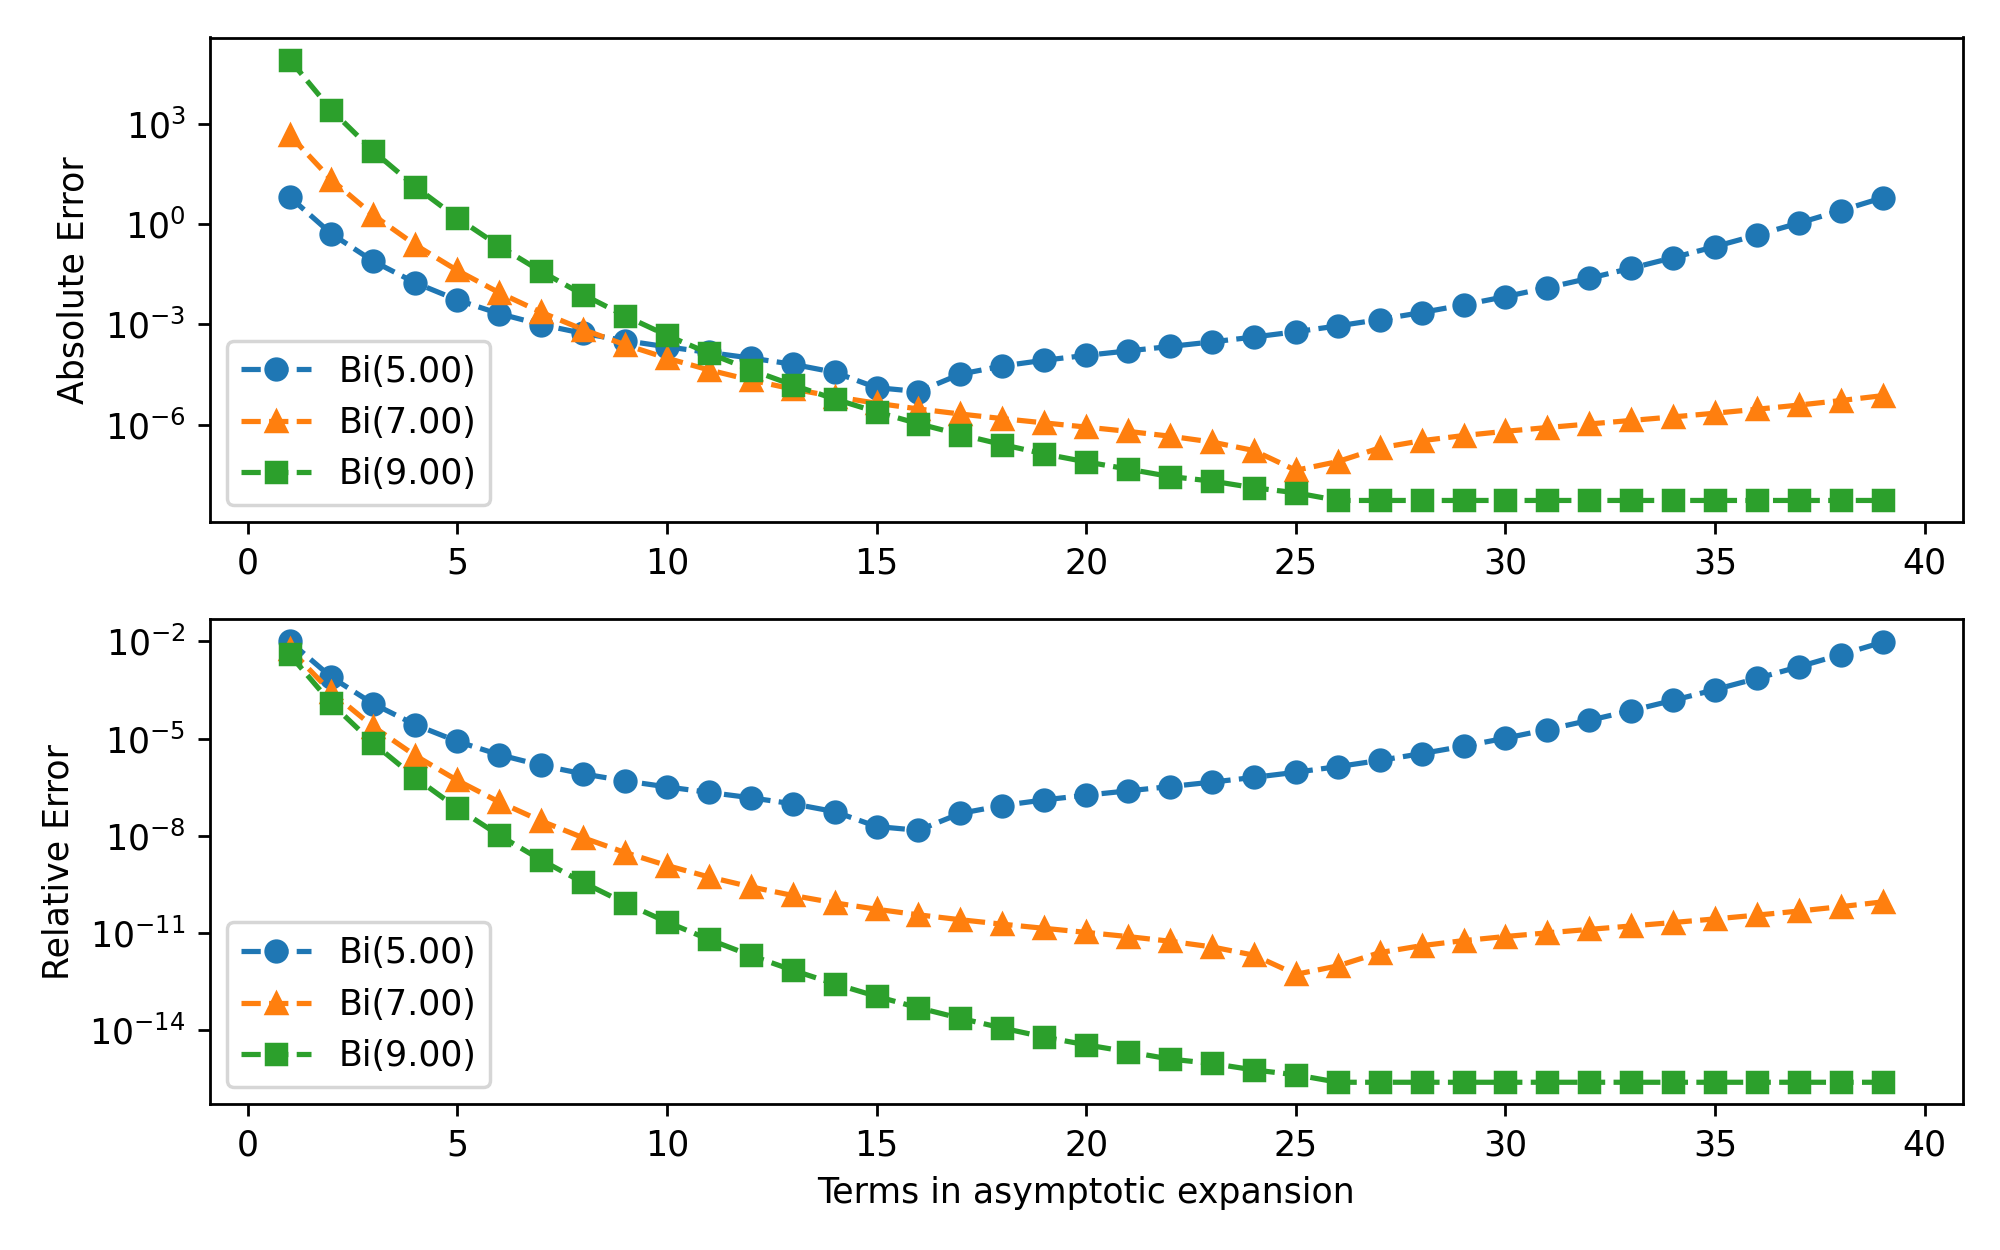
\includegraphics[width=\linewidth]{asymptotic-term-optimization}
	\vspace{-8mm}
	\caption{Absolute and relative error of $ \Bi(x)$ for positive $ x $ as a function of the number of terms in the asymptotic expansion. Note that for small $ x $, adding terms causing error to increase, as expected for an asymptotic series.} 
	\label{airy:fig:asym-optimization}
\end{figure}

\subsubsection{Truncating the Asymptotic Series}
I truncated the series for $ L(x), P(x) $ and $ Q(x) $ (see Equations \ref{airy:eq:LPQ}) using three conditions:
\begin{enumerate}
	\item If subsequent terms differed by less than $ 10^{-16} $. Why so much lower than $ 10^{-10} $? I wanted to push the limits of the accuracy I could achieve, and $ 10^{-16} $ reduced both absolute and relative error in the large $ x $ regime by multiple orders of magnitude compared to $ 10^{-10} $.
	
	\item If subsequent terms in the expansion began to increase, indicating divergence. This applied largely to the smaller values of $ \abs{x} $ in the asymptotic regime; see Figure \ref{airy:fig:asym-optimization}.
	
	\item If the calculation reached 40 terms in the asymptotic expansion. This rarely happened; terms began to differ by less than $ 10^{-16} $ after 20-30 iterations for large $ \abs{x} $. 

\end{enumerate}
I feel like there's enough code already, so I'm leaving out this example; the syntax and logic is analogous to the Maclaurin truncation implementation given above.

\subsection{Switching Between Asymptotic and Maclaurin Regimes}
Obviously, the asymptotic series better approximate $ \Ai $ and $ \Bi $ for large $ \abs{x} $, while the Maclaurin series works better for small $ \abs{x} $. I chose the breakpoints between regimes so that error as a function of $ x $ changed continuously across the transition. I couldn't find a single satisfactory value for the Maclaurin-to-asymptotic transition for positive $ x $, so I implemented separate breakpoints for $ \Ai $ and $ \Bi $. The implementation I used is:
\begin{myminted}
asym_to_power = -7     # from negative asymptotic to Maclaurin
power_to_asym_A = 5.5  # from Maclaurin to positive asymptotic for Ai
power_to_asym_B = 8.2  # from Maclaurin to positive asymptotic for Bi

if x <= asym_to_power:                         # asymptotic for both A and B
    # calculate Ai and Bi...
elif asym_to_power < x <= power_to_asym_A:     # power for both A and B
	# calculate Ai and Bi...
elif power_to_asym_A < x <= power_to_asym_B:   # asymptotic for A and power for B
    # calculate Ai and Bi...
elif x > power_to_asym_B:                      # asymptotic for both A and B
    # calculate Ai and Bi...

\end{myminted}

\begin{figure} [htb!]
	\centering
	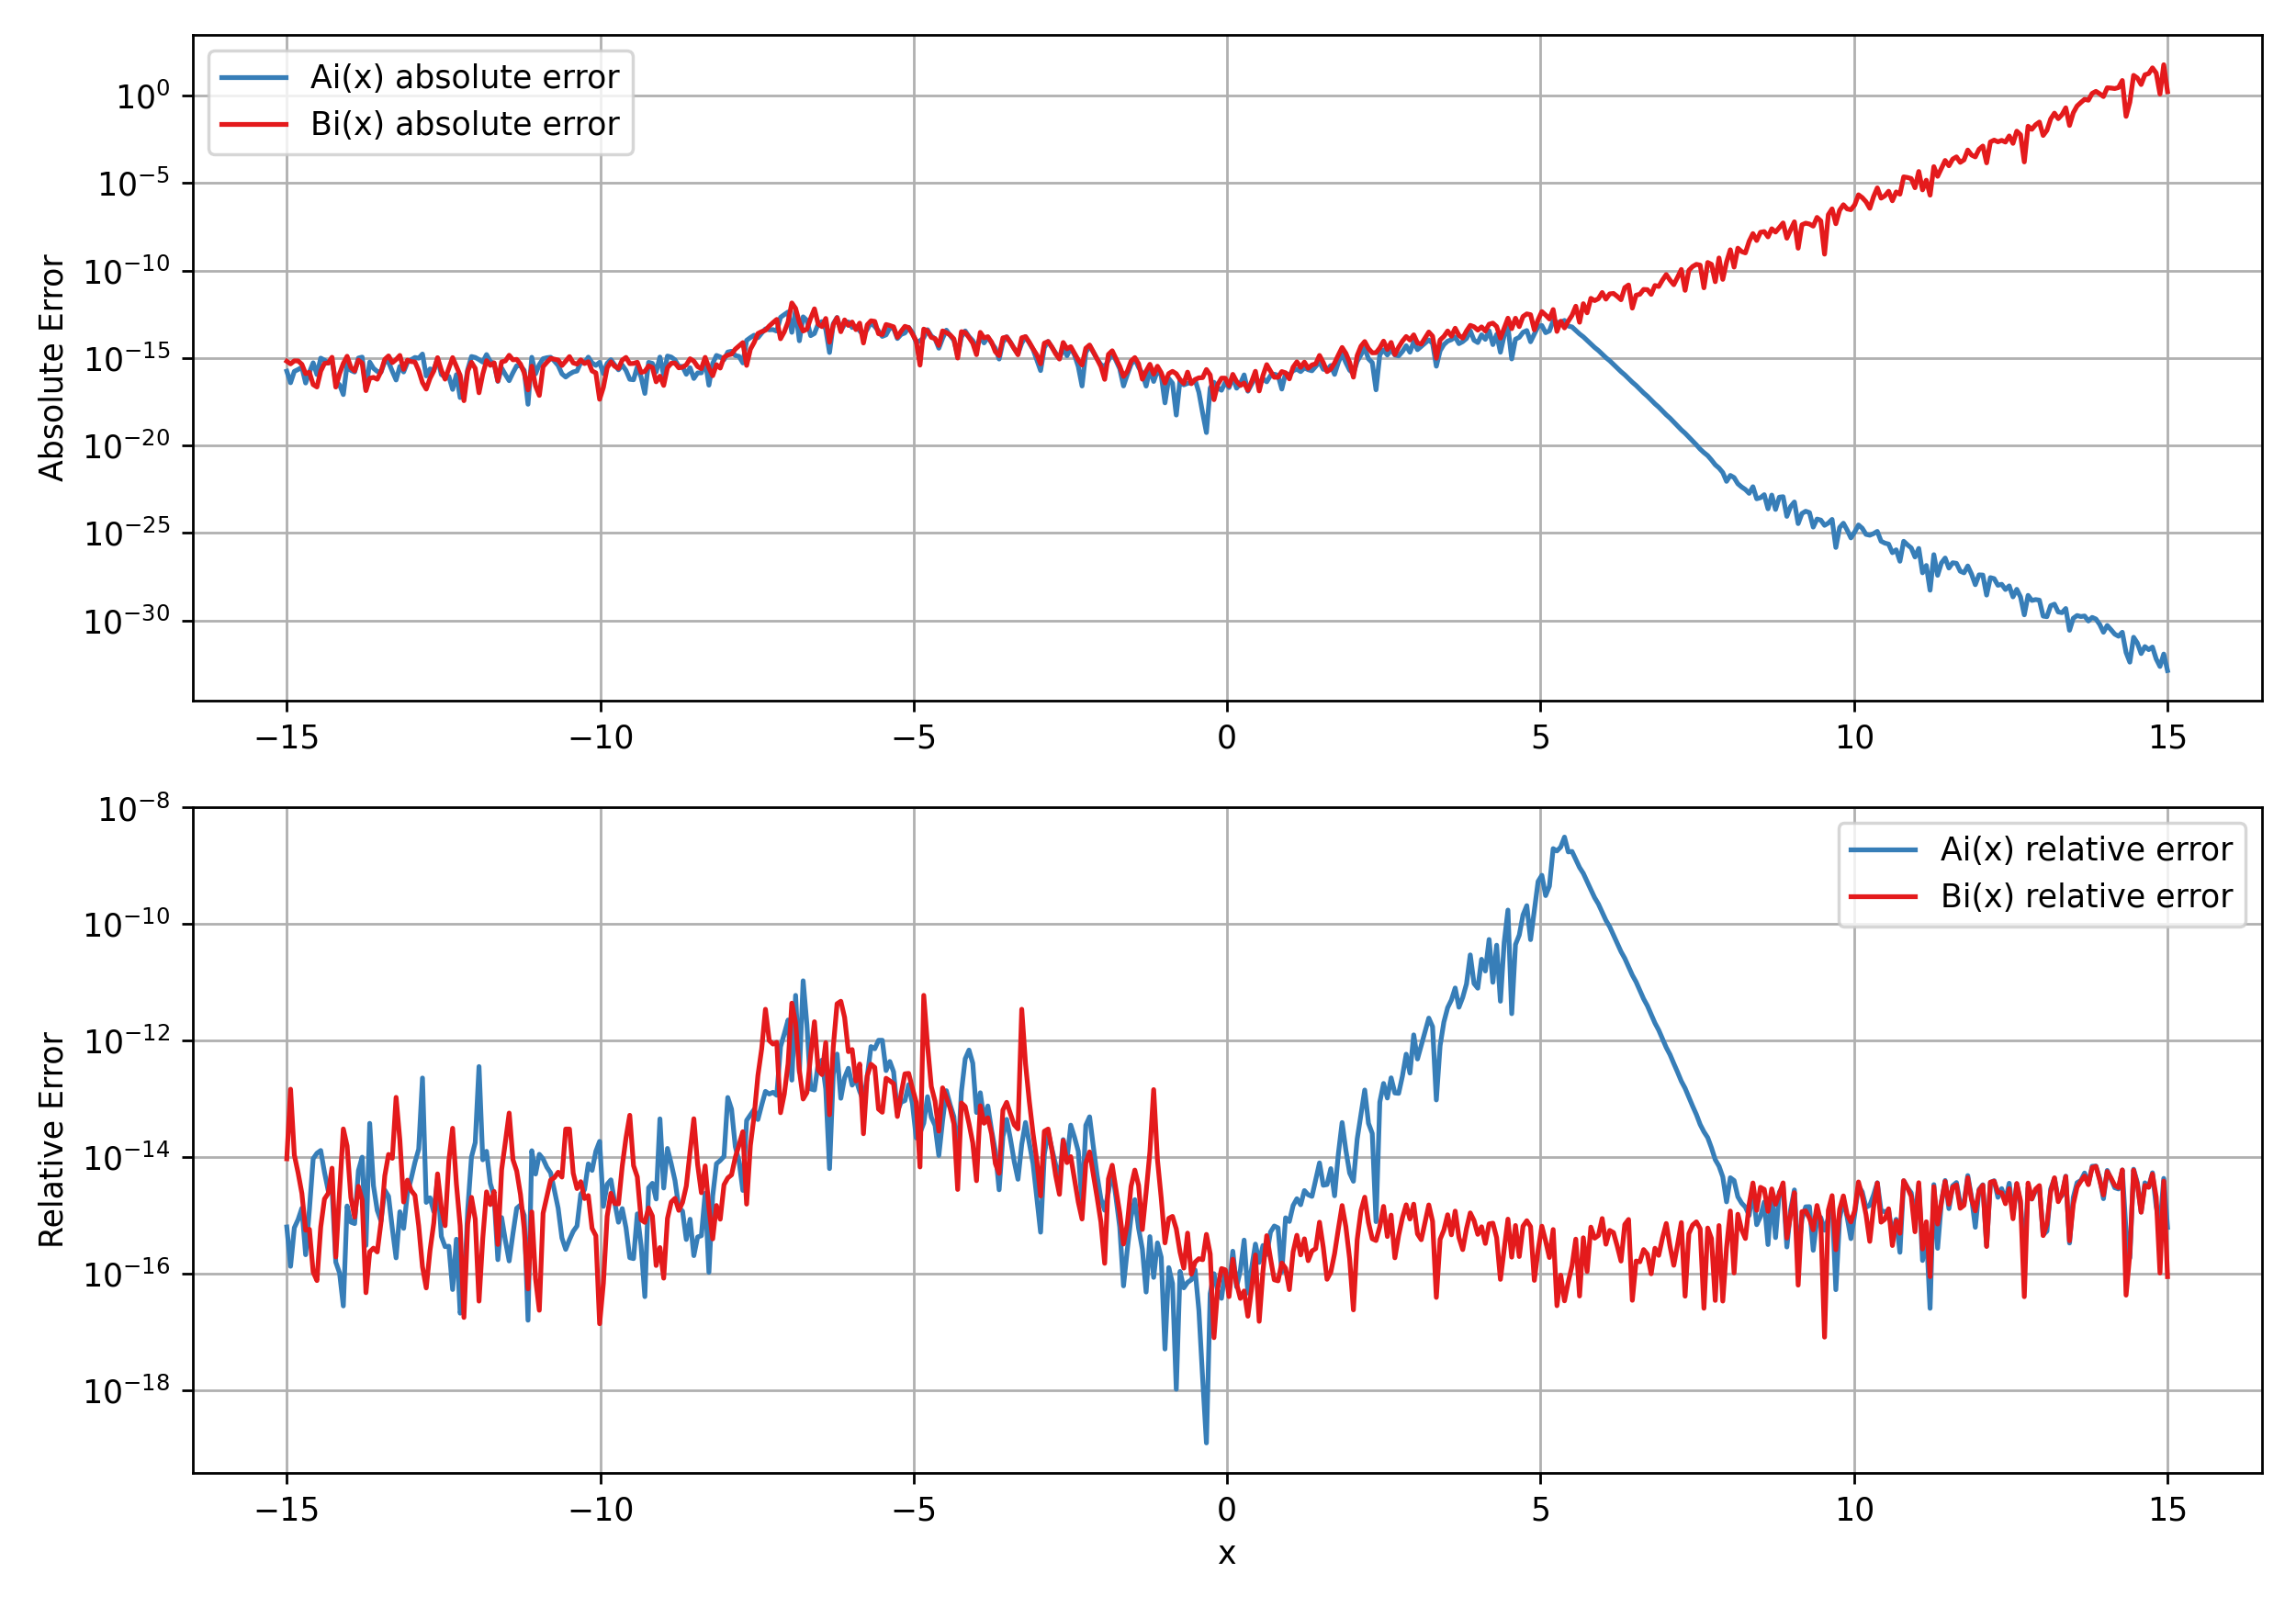
\includegraphics[width=\linewidth]{rel-abs-errors}
	\vspace{-8mm}
	\caption{Relative and absolute error of my implementation of the functions $ \Ai $ and $ \Bi $. Both relative and absolute error stay well below $ 10^{-10} $ for negative $ x $, but absolute error for $ \Bi $ diverges for large $ x $. See \hyperref[airy:ss:results]{\underline{Subsection \ref{airy:ss:results}}} for a more thorough discussion.} 
	\label{airy:fig:rel-abs-errors}
\end{figure}



\subsection{Evaluating Error}
Figure \ref{airy:fig:rel-abs-errors} shows the relative and absolute errors of my implementation of $ \Ai $ and $ \Bi $. 

I used \texttt{mpmath}'s arbitrary precision \texttt{airyai} and \texttt{airybi} functions as the ``true'' value of the Airy functions when evaluating the error of my own implementation. I set \texttt{mpmath} to use 18 decimal places, corresponding to a mantissa precision of 63 bits, compared to the 52-bit mantissa precision of IEEE 745 double-precision values. I could have used higher precision as a better reference, but that seems superfluous, since a 63-bit mantissa is already well-above the 52-bit precision  floating-point arithmetic I am working with.

\begin{figure}
	\centering
	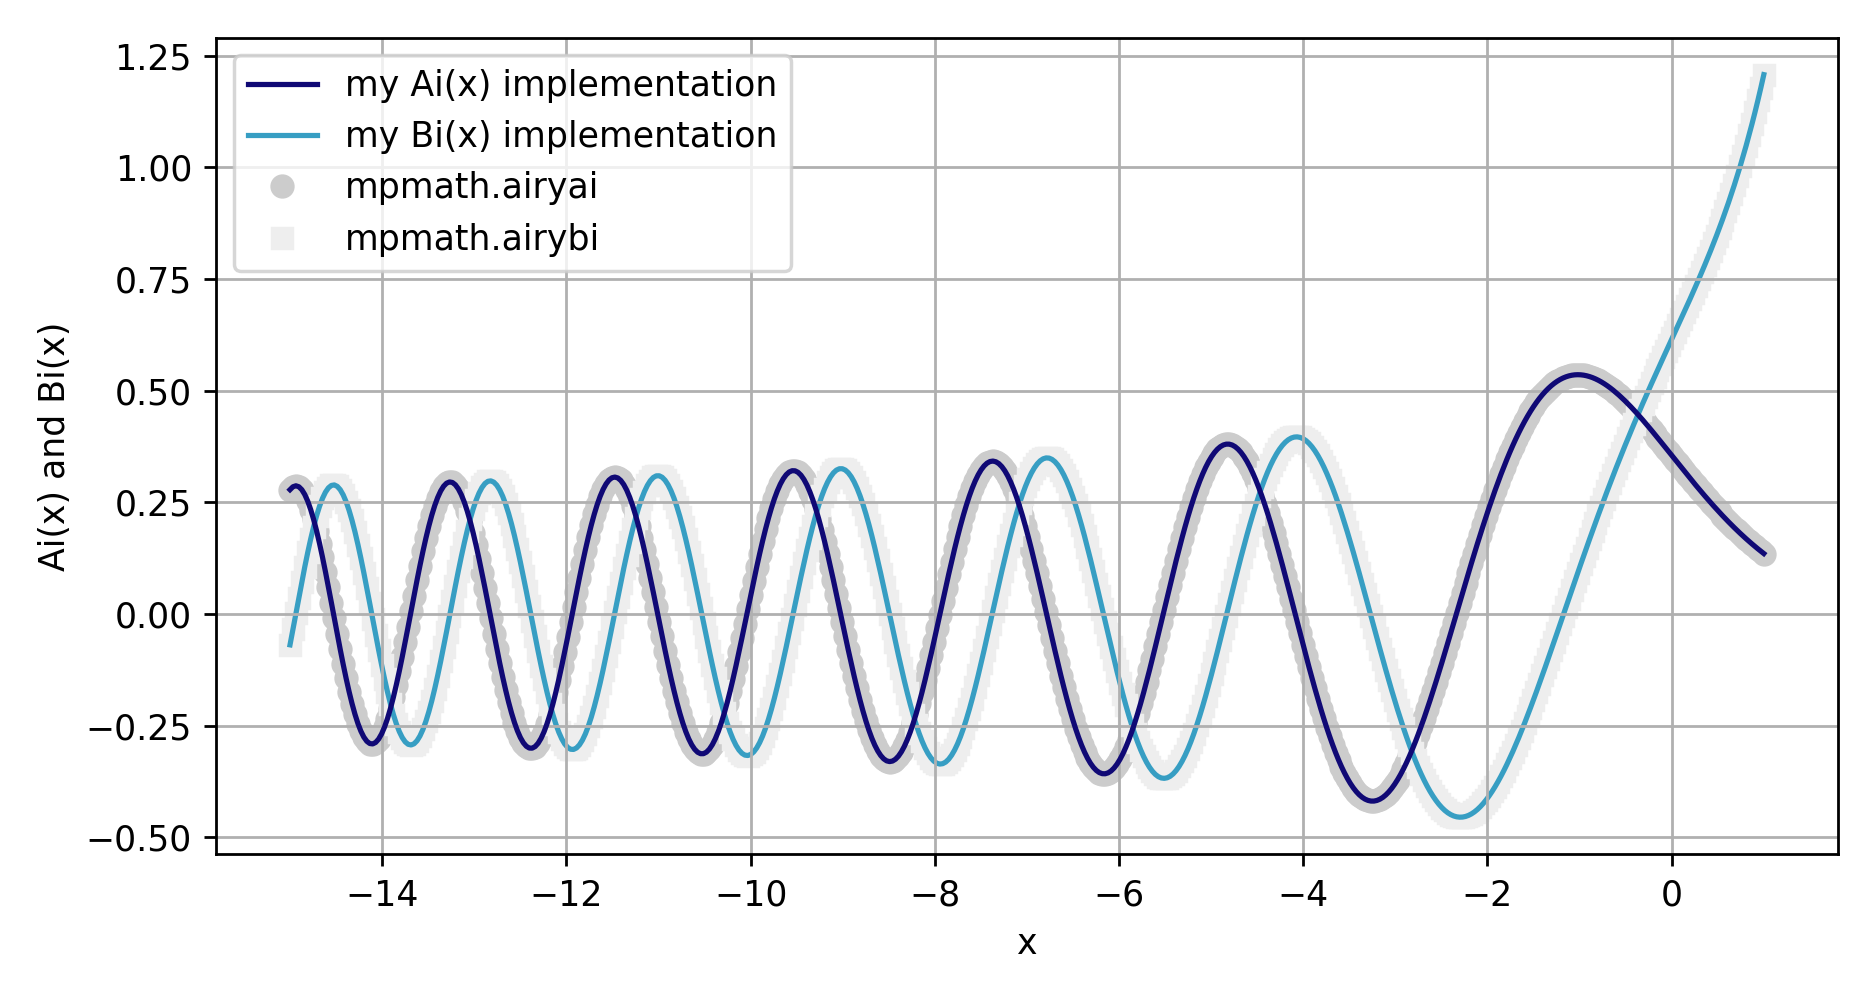
\includegraphics[width=\linewidth]{Ai-Bi-graphs}
	\vspace{-8mm}
	\caption{Graphs of my implementation of $ \Ai $ and $ \Bi $ with arbitrary precision values from \texttt{mpmath.airyai} and \texttt{mpmath.airybi} for reference.} 
	\label{airy:fig:Ai-Bi-graphs}
\end{figure}

\subsection{Results and Takeaway} \label{airy:ss:results}
Figure \ref{airy:fig:Ai-Bi-graphs} shows the graphs of the $ \Ai $ and $ \Bi $ implementation for $ x \in [-15, 1] $. 

Reflecting on the results summarized in Figures \ref{airy:fig:rel-abs-errors} and \ref{airy:fig:Ai-Bi-graphs}, I'm satisfied with:
\begin{itemize}
	\item Absolute and relative error in the asymptotic regime of large negative $ x $, which are both comfortably below $ 10^{-10} $.
	
	\item Absolute error of the Maclaurin series for small $ \abs{x} $, which remains comfortably below $ 10^{-10} $ in the Maclaurin regime.
	
	\item Aside from a slight divergence for $ \Ai $ near the positive Maclaurin-to-asymptotic transition (discussed below), relative error in both $ \Ai $ and $ \Bi $ remains below $ 10^{-10} $ over the entire real line.
	
\end{itemize}


I'm not satisfied with: 
\begin{itemize}
	\item For $ \Ai(x) $, relative error climbs to roughly $ 3\cdot 10^{-9} $ in the neighborhood of the transition point $ x = 5.5 $ both in the Maclaurin and asymptotic approximations. I aimed to keep relative error below $ 10^{-10} $ over the entire real line, and was unsuccessful because of this trouble spot.
	
	\item Divergence of the absolute error of $ \Bi(x) $ for large positive $ x $, which means I was unsuccessful in the the assignment, which called for absolute error below $ 10^{-10} $ over the entire real line. This error divergence appears to be a consequence of finite-precision floating-point arithmetic, which becomes problematic as $ \Bi $ diverges towards $ + \infty $. It is worth noting, however, that relative error of $ \Bi $ remains well below $ 10^{-10} $ over the entire real line.
	

	
\end{itemize}


\section{Zeros}
I calculated the Airy functions' zeros using three methods:
\begin{enumerate}
	\item The arbitrary precision \texttt{mpmath} functions \texttt{airyaizero(n)} and \texttt{airybizero(n)}, which return $ \Ai $ and $ \Bi $'s $ n $th zero, respectively, to arbitrary precision. 
	
	\item The asymptotic formula given in Equation \ref{airy:eq:zeros}.
	
	\item My own algorithm using the bisection method and my implementation of $ \Ai $ and $ \Bi $.
\end{enumerate}

\subsection{Asymptotic Zero Algorithm}
I directly implemented Equation \ref{airy:eq:zeros}. The implementation is straightforward and I think including code would be overkill. The only detail worth mentioning is that for the first zero, I truncated the asymptotic series at the fourth term for $ \Ai $ and the second term for $ \Bi $ to minimize error. This improved the accuracy by roughly one and two orders of magnitude, respectively.

\begin{figure}[htb!]
	\centering
	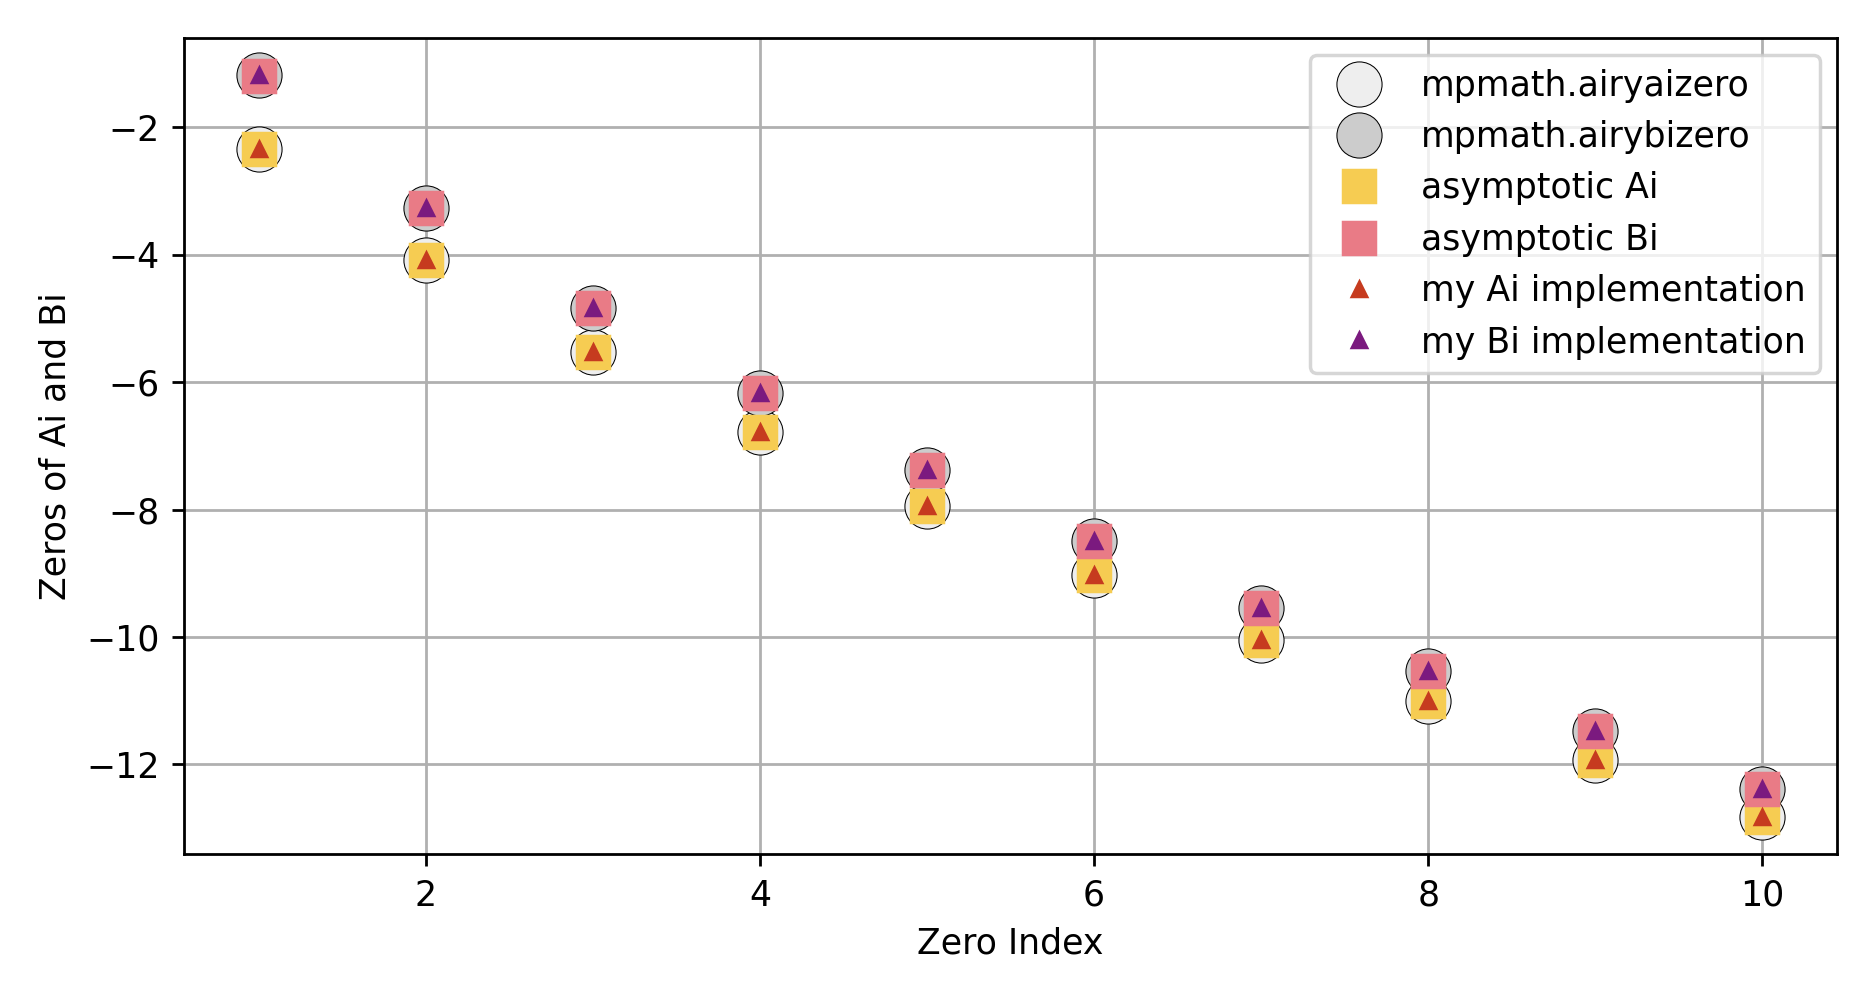
\includegraphics[width=\linewidth]{zeros-compared}
	\vspace{-8mm}
	\caption{The first 10 zeros of $ \Ai $ and $ \Bi $ found using \texttt{mpmath.airyzero}, the asymptotic formula from Equation \ref{airy:eq:zeros} and my bisection method implementation from \hyperref[airy:ss:zero-algorithm]{\underline{Subsection \ref{airy:ss:zero-algorithm}}}. Only 10 zeros are shown to reduce clutter; for the full 100 zeros see Figure \ref{airy:fig:zero-erors}.}
	\label{airy:fig:zeros-compared}
\end{figure}


\subsection{My Attempt at a Zero-Finding Algorithm} \label{airy:ss:zero-algorithm}
The algorithm actually works satisfactorily. It can be abstracted into three steps:
\begin{enumerate}
	\item Calculate Airy function values on the interval containing the desired number of zeros, e.g. $ [-61, 0] $ for the first 100 zeros, using my Airy function implementation.
	
	\item Loop through the Airy function values and detect when the values change sign, meaning there is a zero in the interval between the two function values. Store the $ x $ values of the interval endpoints in an array.	
	
	The sample rate of the function values must be large enough to have at least one point between each zero---500 points is more than enough to cover the first 100 zeros.
	
	\item Loop through the array of intervals containing zeros and find each zero using the bisection method: pass the left and right endpoints as arguments, specify a tolerance, and calculate function values using my Airy function implementation.
	
\end{enumerate}


In Python, a possible implementation of the bisection zero algorithm reads
\begin{myminted}
max_zeros = 100                     # find 100 zeros
eps = 1e-8                          # tolerance for bisection method
X = np.linspace(-65, 0, 500)        # sample 500 points between -65 and 0
my_ai_values = get_my_ai_values(X)	# calculate values of Ai on X
current_value = my_ai_values[0]     # value of Ai at first point
zero_intervals = []   # intervals representing the two closest points to each zero
zero_counter = 0      # counts how many zeros have been found
for i in range(1, numpoints):  # loop through Airy function values
    prev_value = current_value         # store previous value
    current_value = my_ai_values[i]    # update current value

    if zero_counter < max_zeros and ((prev_value <= 0 <= current_value) or (current_value <= 0 <= prev_value)):  # crossed a zero
        zero_intervals.append((X[i-1], X[i]))  # record interval containing zero
        zero_counter += 1                      # update zero counter

my_airyaizeros = []                       # array to store zeros
for i in range(0, len(zero_intervals)):   # loop through array of zero intervals
    zero = bisection(my_airyai, zero_intervals[i][0], zero_intervals[i][1], eps)
    my_airyaizeros.append(zero)   # calculate zero with bisection, store in array
\end{myminted}

The bisection implementation I used is:
\begin{myminted}
def bisection(f, a, b, eps):
    if a == 0.0: return a   # safety check in case endpoints are zeros
    if b == 0.0: return b
	
    counter = 0
    max_iterations = 100  # infinite loop protection; never reached in practice
    while abs(b-a) > eps:
        c = a + (b-a)/2   # less risk of overflow than (a+b)/2
        
        if np.sign(f(a)) == np.sign(f(c)): a = c   # shift left endpoint to c
        else: b = c                                # shift right endpoint to c
        counter += 1
        if counter > max_iterations: break  # infinite loop protection

    return a + (b - a)/2

\end{myminted}
The algorithm's accuracy depends largely on the tolerance $ \epsilon $ used with the bisection method, as seen in Figure \ref{airy:fig:zero-erors}. Of course, the accuracy can be no better than the accuracy of my Airy function implementation, which has an absolute error of about $ 10^{-15} $ for large negative $ x $.

Figure \ref{airy:fig:zero-erors} includes a run of the bisection method with an excessively small tolerance of $ \epsilon = 10^{-20} $. This is done intentionally to demonstrate that floating-point precision limits the algorithm's accuracy to about $ 10^{-16} $, regardless how small I make $ \epsilon $. 

\vspace{-3mm}
\begin{figure}[htb!]
	\centering
	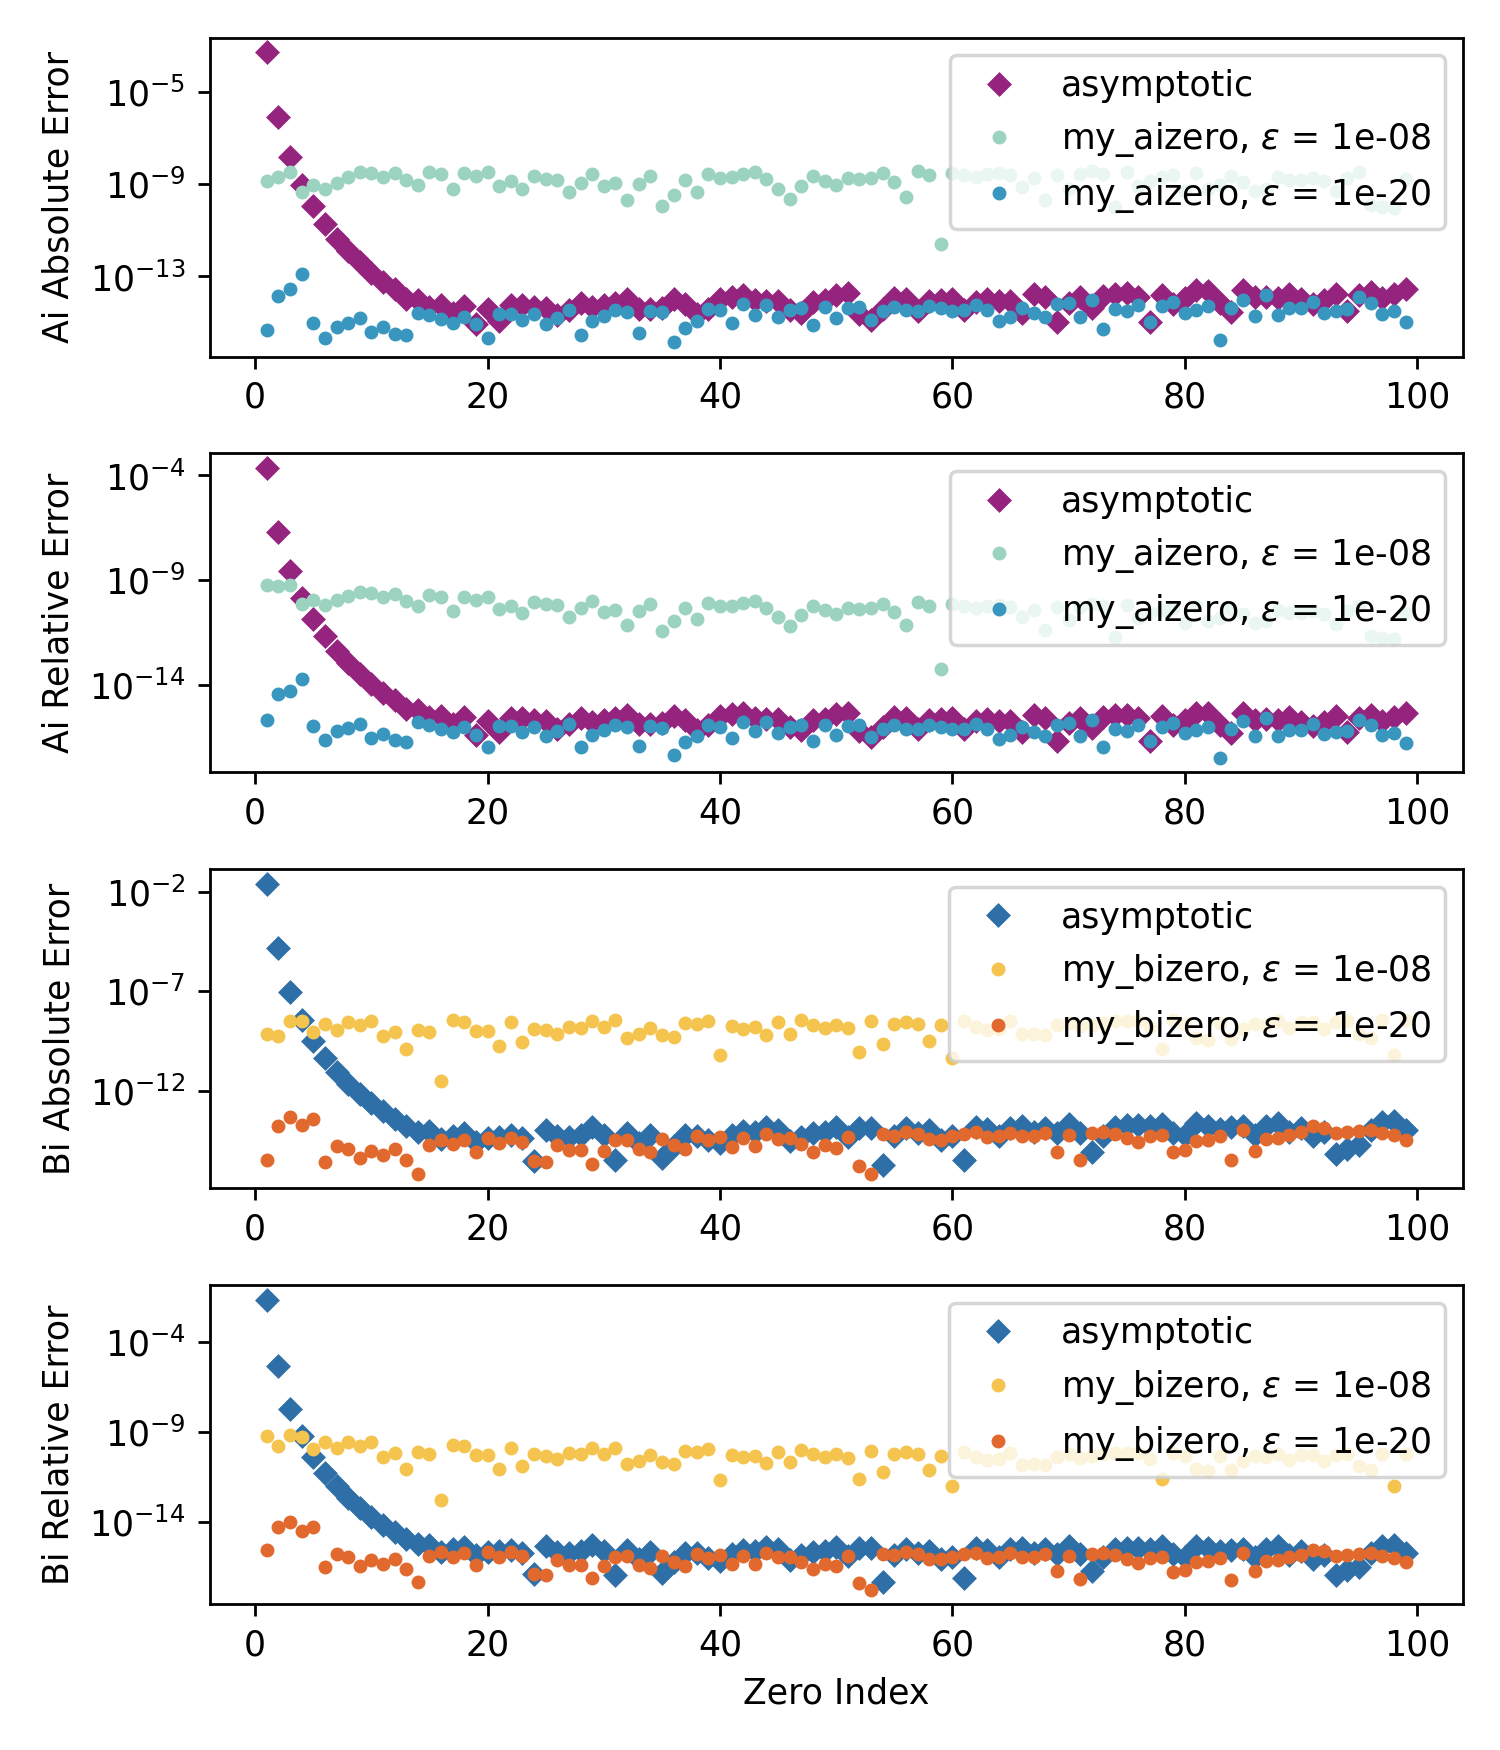
\includegraphics[width=.95\linewidth]{zero-errors}
	\vspace{-8mm}
	\caption{Absolute and relative errors of the first 100 zeros of $ \Ai $ and $ \Bi $ using the asymptotic formula from Equation \ref{airy:eq:zeros} and two runs of my own bisection method implementation, discussed in \hyperref[airy:ss:zero-algorithm]{\underline{Subsection \ref{airy:ss:zero-algorithm}}}. The accuracy of the asymptotic approximation exponentially improves with increasing zero index, while the bisection implementation accuracy is a largely constant function of bisection tolerance $ \epsilon $. \textit{The second bisection run with excessively low $ \epsilon = 10^{-20} $ shows that floating-point precision limits accuracy to about $ 10^{-15} $.}}
	\label{airy:fig:zero-erors}
\end{figure}

\vspace{-5mm}

\end{document}



